% ============================================================
%  Overleaf-ready. Compiles with pdfLaTeX.
%  UPLOAD the six figures into a folder called  figures/  in your
%  Overleaf project (same names as below):
%    figures/panels_2024.png
%    figures/roc_cv.png
%    figures/change_map.png
%    figures/lst_by_class_year.png
%    figures/day_vs_night_effect.png
%    figures/core_vs_fringe_night.png
% ============================================================
\documentclass[11pt]{article}

\usepackage[utf8]{inputenc}
\usepackage[T1]{fontenc}
\usepackage[margin=1in]{geometry}
\usepackage{graphicx}
\usepackage{booktabs}
\usepackage{amsmath}
\usepackage{caption}
\usepackage{enumitem}
\usepackage[hidelinks]{hyperref}

% degrees Celsius that works in text and math
\newcommand{\dC}{\ensuremath{\,^{\circ}\mathrm{C}}}

\title{\vspace{-1.5em}A Satellite AI Model Maps Addis Ababa's Informal
Settlements --- and Finds a Heat Penalty Hidden Until Nightfall
(2017--2024)}
\author{Nahom Azmach}
\date{Draft: 70 hand-digitized labels; daytime + nighttime thermal analysis}

\begin{document}
\maketitle

% ---------------- Key terms box ----------------
\begin{quote}
\small
\textbf{Key terms}
\begin{description}[leftmargin=1em, itemsep=2pt]
  \item[Informal settlement:] densely built, unplanned housing --- in Addis,
  typically small corrugated-metal-roofed dwellings on narrow, irregular
  streets (``slum'' fabric), as opposed to planned apartments, villas, and
  industrial areas (``formal'').
  \item[Satellite embedding / foundation model:] an AI model trained on
  enormous amounts of imagery that turns each patch of ground into a list of
  numbers summarizing what's there. Just as a language model turns a sentence
  into numbers that capture its meaning, \textbf{AlphaEarth} turns every
  10-metre patch of Earth into \textbf{64 numbers}. You don't hand-code what
  to look for --- the model already learned general visual features.
  \item[LST (land-surface temperature):] how hot the physical surface (roofs,
  roads, soil) is, read by a thermal satellite. \emph{Not} the same as the
  air temperature a person feels.
  \item[NDVI:] a standard ``greenness'' score from satellite bands; high =
  lush vegetation, low = bare or built-up.
  \item[Landsat vs MODIS:] two thermal satellites. \textbf{Landsat} is sharp
  (30 m) but only passes over in mid-morning. \textbf{MODIS} is coarse (1 km)
  but passes several times a day --- including $\sim$1:30 am --- so it can
  measure \textbf{night}.
  \item[Adjusted effect:] a temperature difference between the two fabric
  types \emph{after} using regression to statistically remove the influence of
  elevation and greenery, so what's left is attributable to the fabric itself.
\end{description}
\end{quote}

% ---------------- Abstract ----------------
\begin{abstract}
Every recent study of Addis Ababa's urban heat relies on hand-crafted formulas
applied to satellite bands (indices like NDVI/NDBI) plus standard regression,
and none is framed around fairness to informal settlements. I take a different
approach: I let an AI \textbf{satellite foundation model} (AlphaEarth) describe
the ground, train a simple classifier on its output to tell informal from
formal fabric, and then compare the two on temperature. Trained once on 2024
labels and applied to both 2017 and 2024, the classifier separates the two
fabrics well (\textbf{cross-validated AUC 0.938} --- see Section~\ref{sec:clf})
and maps clear settlement expansion at the city's edges. Surprisingly, by
\textbf{day} informal fabric is \textbf{not} hotter --- after accounting for
elevation and greenery it is slightly \emph{cooler} ($-0.41$\dC{} in 2017,
$-0.38$\dC{} in 2024). But when I extend the analysis to \textbf{night} (using
MODIS), the picture inverts: in 2017 informal fabric is significantly
\emph{hotter} after dark ($+0.30$\dC{} per pixel; \textbf{$+1.13$\dC} in a
cleaner ``pure-cell'' test, $p \approx 10^{-11}$), and the nighttime penalty
concentrates in the \textbf{established dense core} ($+0.34$\dC) rather than the
newly-expanded fringe. The daytime null was an artifact of \emph{when} the
satellite looks: \textbf{daytime surface temperature hides a heat penalty that
is real at night}, when dense fabric releases stored heat and residents cannot
cool down. The AI classifier is a clear step up from index-based mapping; the
day-vs-night contrast is the substantive contribution.
\end{abstract}

% ---------------- 1. Introduction ----------------
\section{Introduction}
Urban heat is a fairness problem: the people least able to adapt often live
where it is hottest. Addis Ababa is growing fast, and its informal settlements
are spreading into the peri-urban fringe (the edge where city meets
countryside). Recent studies measure the city's ``urban heat island,'' but they
stop at index-based regression and none isolates an informal-settlement effect
or asks whether the gap is widening.

This project asks: \textbf{can an AI satellite model detect informal fabric and
any linked heat signal --- without hand-crafted indices --- and track how it
changes as settlements grow?} The contributions are:
\begin{enumerate}[leftmargin=1.4em, itemsep=1pt]
  \item The first use of a satellite foundation model (AlphaEarth) to map Addis
  Ababa's urban fabric.
  \item A confounder-adjusted estimate of the informal-vs-formal temperature
  difference, using a \emph{train-once/apply-twice} design for an honest
  2017$\rightarrow$2024 comparison.
  \item A \textbf{daytime-vs-nighttime} comparison showing the heat penalty is
  invisible by day but present at night --- a concrete demonstration that
  \emph{when} you measure decides whether you see the inequity at all.
  \item A \textbf{core-vs-fringe} breakdown locating that nighttime penalty in
  the established settlement rather than the expanding frontier.
\end{enumerate}

% ---------------- 2. Related Work ----------------
\section{Related Work}
Existing Addis heat studies use greenness/built-up indices with ordinary or
geographically-weighted regression, or split results by building type. None
uses learned AI representations or an explicit informal-settlement fairness
frame. AlphaEarth Foundations (the model used here) introduces the annual
10 m, 64-number embeddings and shows that even \emph{simple} classifiers on
them match or beat purpose-built models. Machine-learning mapping of deprived
areas in Accra, Lagos, and Nairobi, and a deprivation study of Addis, guide
where informal fabric concentrates.

% ---------------- 3. Data ----------------
\section{Data}
\begin{table}[htbp]
\centering
\small
\begin{tabular}{@{}llll@{}}
\toprule
Layer & Source & Resolution & Role \\
\midrule
Land description & AlphaEarth Satellite Embedding V1 & 10 m, 64 numbers & Classifier input \\
Surface temp (day) & Landsat 8/9 surface temp. & 30 m $\rightarrow$ 10 m & Outcome \\
Surface temp (day+night) & MODIS Terra+Aqua LST & 1 km & Outcome (extension) \\
Greenness & Sentinel-2 NDVI & 10 m & Control variable \\
Elevation & SRTM & 30 m & Control variable \\
Built-up mask & GHS-BUILT-S (2025) & 100 m & Study-area definition \\
RGB photo & Sentinel-2 (true colour) & 10 m & Visualization only \\
\bottomrule
\end{tabular}
\caption{Data layers. All temperatures and indices are dry-season (Dec--Feb)
medians.}
\end{table}

\paragraph{Study area.} The official city boundary ($\sim$542\,km\textsuperscript{2})
is tighter than the real built-up city and cuts off the peri-urban fringe ---
exactly where informal growth happens, and where 27\% of my informal labels
fell. So I define the study area as the official boundary \textbf{grown outward
by 10 km, then trimmed to built-up land only} (using a global settlement
layer). This keeps rural farmland from sneaking into the ``formal'' group and
making it look artificially cool. Everything is composited over the
\textbf{dry season} (Dec--Feb) to avoid rainy-season clouds. The result is
$\sim$420\,km\textsuperscript{2} of city (a 5008$\times$4956-pixel grid at
10 m).

% ---------------- 4. Labels ----------------
\section{Labels}
No ready-made map of Addis's informal settlements exists, so I hand-drew
\textbf{70 polygons} (31 informal / 39 other) over high-resolution 2024
imagery, covering both the inner city and the fringe, guided by neighbourhoods
the deprivation literature flags. I labelled only against 2024 imagery; the
trained model is then applied \emph{unchanged} to 2017 (see Section~\ref{sec:method}).
Sixty-four polygons landed on valid built-up pixels. Crucially, when measuring
accuracy I split \textbf{by polygon, not by pixel} --- pixels from the same
drawn shape look almost identical, so letting them appear in both training and
testing would inflate the score.

% ---------------- 5. Method ----------------
\section{Method}\label{sec:method}
\paragraph{Classifier.} A simple per-pixel model reads the 64 numbers for a
pixel and predicts informal vs other. I compare three: a \textbf{linear} model
(logistic regression), a small \textbf{neural network} (MLP), and
\textbf{gradient-boosted trees} (XGBoost). Accuracy is measured with
\emph{polygon-grouped 5-fold cross-validation} --- the data is split into five
groups of whole polygons, and each group takes a turn being the held-out test
set, so every polygon is predicted by a model that never saw it.

\paragraph{Train once, apply twice.} I train on 2024 labels, then \emph{freeze}
the model and run it on both 2017 and 2024 imagery. Because the decision rule
never changes, any difference between years reflects real change on the ground,
not me labelling differently. Pixels that flip from ``other'' (2017) to
``informal'' (2024) form the \textbf{settlement-expansion map}.

\paragraph{Statistics.} For each year I compare the two classes' temperatures
with a Mann--Whitney U test (a rank-based test that doesn't assume a bell
curve) and, more importantly, a regression
\texttt{LST \textasciitilde{} class + NDVI + elevation}. The coefficient on
\texttt{class} is the \textbf{adjusted effect}: the leftover temperature gap
attributable to fabric type after removing greenery and elevation. A pooled
model with a \texttt{class} $\times$ \texttt{year} term tests whether the gap
changed over time, and I cross-check by comparing classes \emph{within} narrow
elevation bands.

\paragraph{Nighttime extension.} I repeat the adjusted regression using MODIS
\textbf{night} temperature (with MODIS \textbf{day} as a same-satellite
control). Because MODIS pixels are $\sim$1 km and informal patches are often
smaller, one pixel can mix both fabrics; so I add (a) a \textbf{purity-restricted}
test using only 1 km cells that are $\geq$70\% one class, and (b) a
\textbf{core-vs-fringe} split that labels pure-informal cells as established
\emph{core} (already informal in 2017) or \emph{expansion} (informal only by
2024) and compares each to \emph{other} cells.

% ---------------- 6. Results ----------------
\section{Results}

\begin{figure}[htbp]
\centering
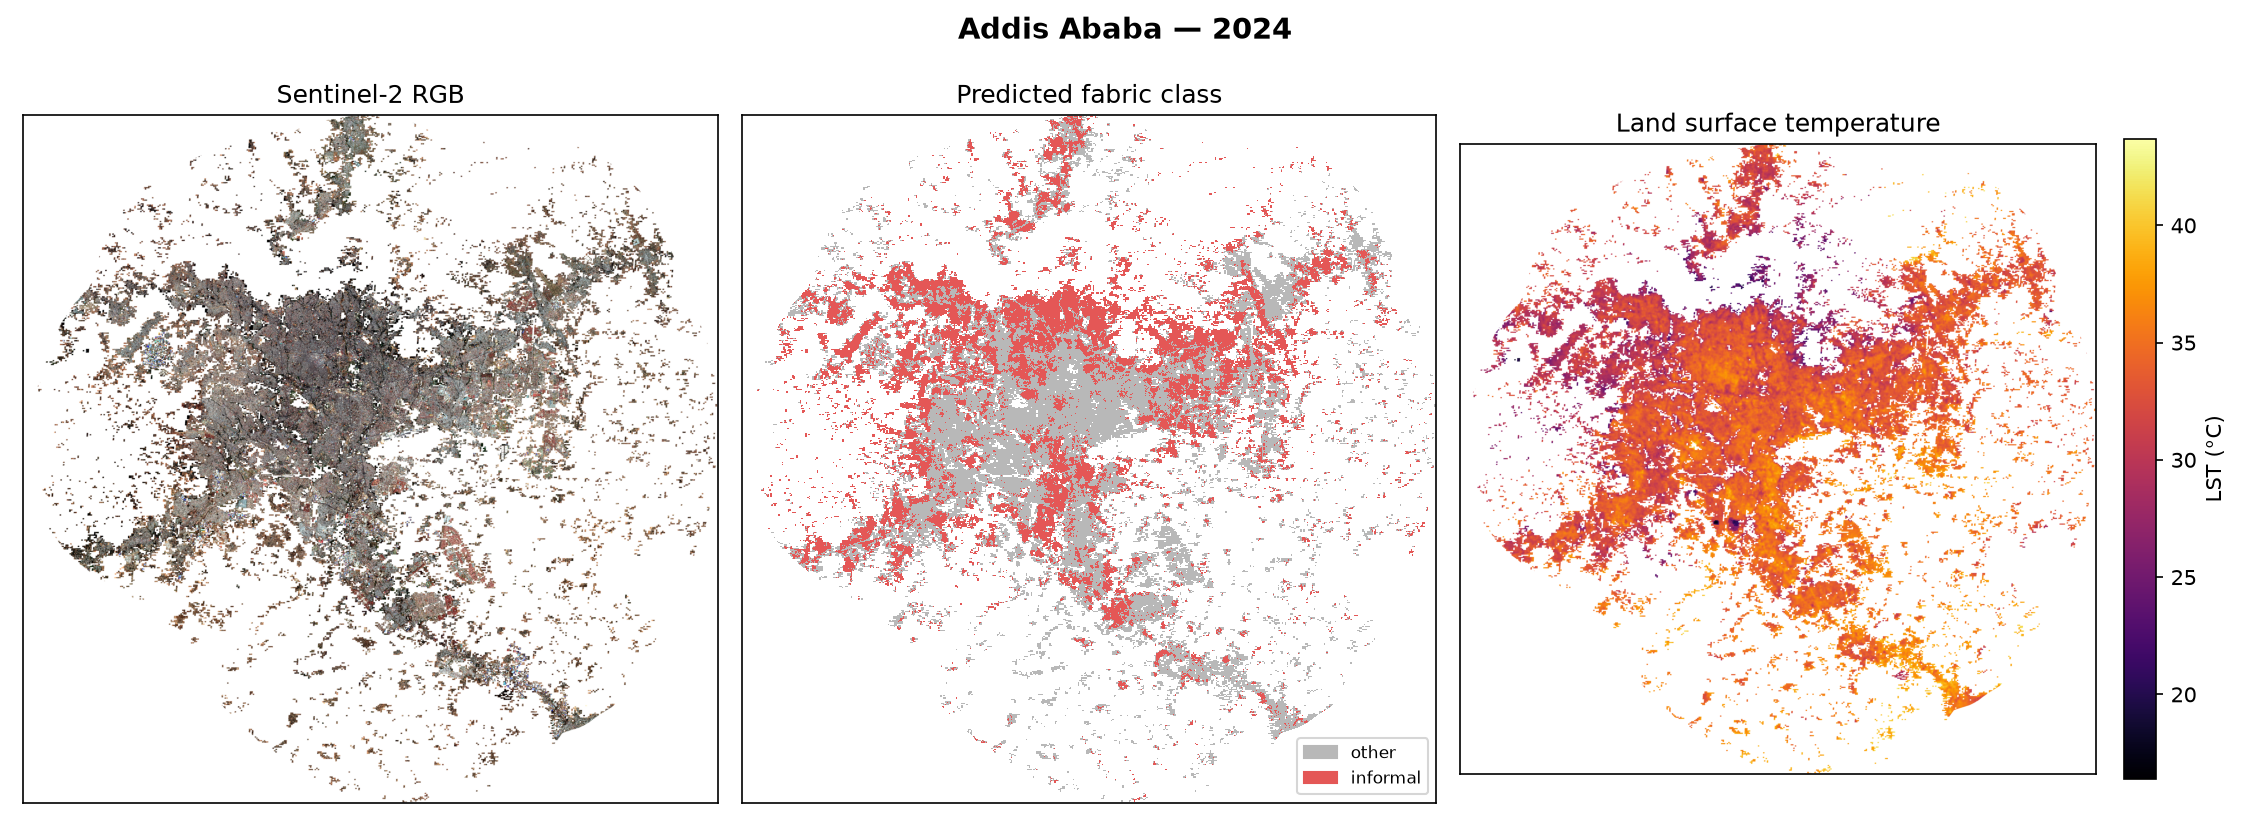
\includegraphics[width=\linewidth]{figures/panels_2024.png}
\caption{The three data views for 2024. Left: true-colour satellite photo.
Centre: the AI classifier's map of fabric type (red = informal, grey = other).
Right: daytime surface temperature. Only built-up land is analysed; white is
outside the study area.}
\end{figure}

\subsection{Classification}\label{sec:clf}
The simple \textbf{linear} model wins --- a known trait of these AI embeddings,
where the useful information is already laid out so plainly that fancy models
add little. (AUC, ``Area Under the Curve,'' scores separation from
0.5 = coin-flip to 1.0 = perfect.)

\begin{table}[htbp]
\centering
\small
\begin{tabular}{@{}lccc@{}}
\toprule
Model & CV AUC & CV F1 & Per-polygon AUC \\
\midrule
\textbf{Logistic regression (linear)} & \textbf{0.938} & 0.853 & 0.935 \\
MLP (neural net) & 0.896 & 0.831 & 0.912 \\
XGBoost (trees) & 0.861 & 0.770 & 0.856 \\
\bottomrule
\end{tabular}
\caption{Classifier comparison under polygon-grouped cross-validation.}
\end{table}

\begin{figure}[htbp]
\centering
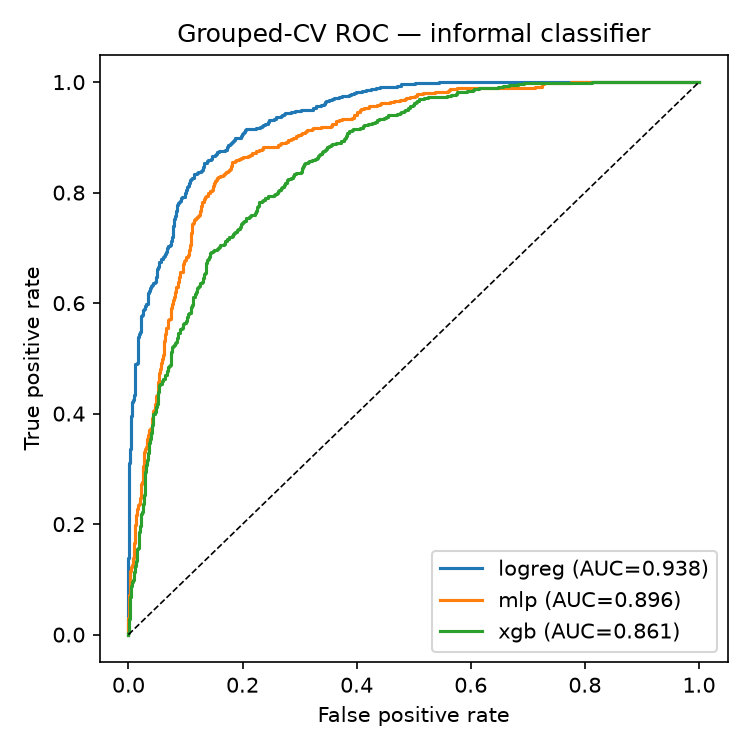
\includegraphics[width=0.62\linewidth]{figures/roc_cv.png}
\caption{How well each model separates informal from other. Higher/closer to
the top-left is better. The linear model (AUC 0.938) leads.}
\end{figure}

The share of built-up land predicted informal rises from
\textbf{31\% (2017) to 42\% (2024)}, and the change map marks \textbf{18\% of
the city as new (other$\rightarrow$informal) growth}, mostly at the fringe ---
the pattern we'd expect from Addis's rapid expansion.

\begin{figure}[htbp]
\centering
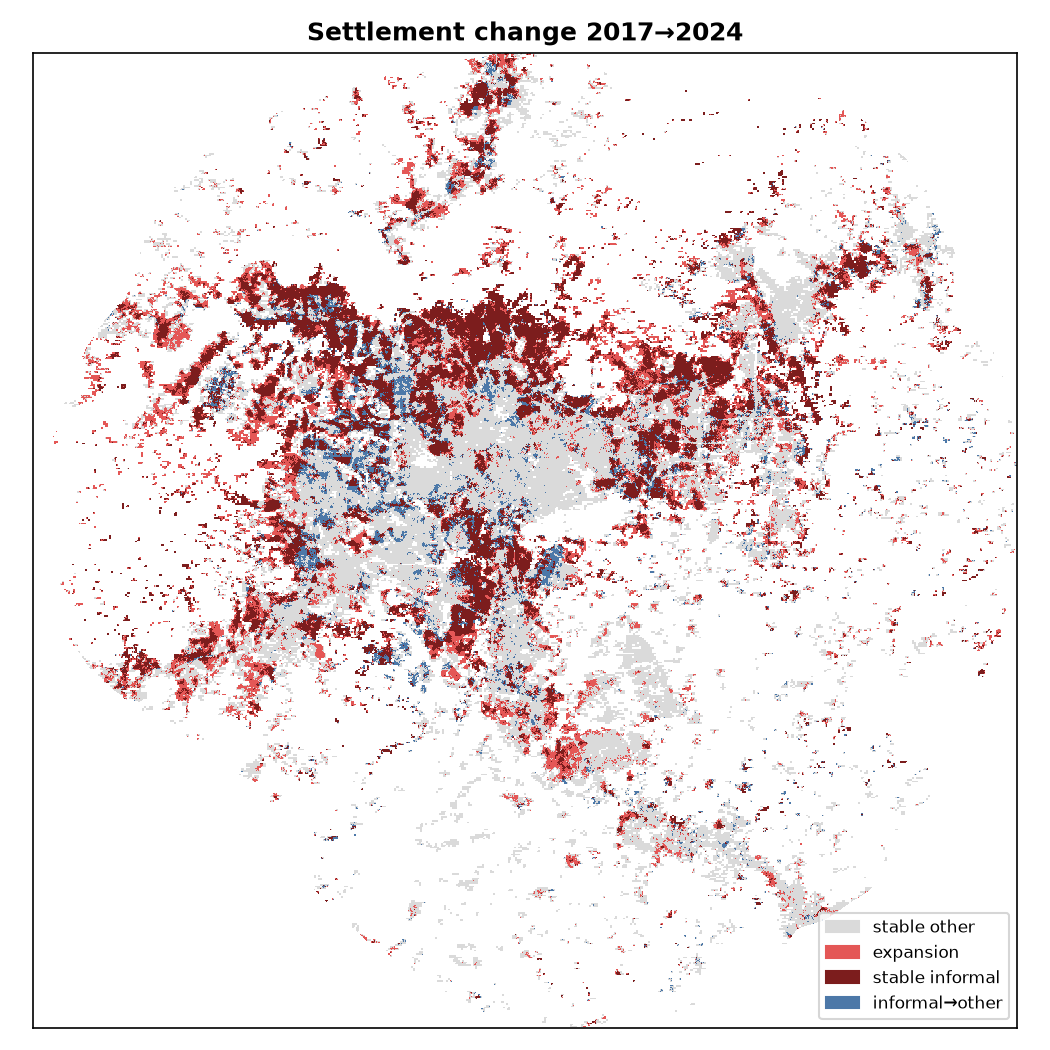
\includegraphics[width=0.5\linewidth]{figures/change_map.png}
\caption{Where the city changed. Red = new informal growth
(2017$\rightarrow$2024); dark red = informal in both years (established core).
Growth clusters at the peri-urban edges.}
\end{figure}

\subsection{The daytime result}
Against expectation, by day informal fabric is \textbf{cooler}, not hotter:

\begin{table}[htbp]
\centering
\small
\begin{tabular}{@{}lcccc@{}}
\toprule
Year & Raw temp gap & Adjusted (greenery+elev.) & 95\% CI & Effect size \\
\midrule
2017 & $-0.76$\dC & \textbf{$-0.405$\dC} & $[-0.433, -0.376]$ & 0.18 \\
2024 & $-0.90$\dC & \textbf{$-0.379$\dC} & $[-0.406, -0.352]$ & 0.25 \\
\bottomrule
\end{tabular}
\caption{Daytime (Landsat) informal-vs-other temperature gap. Negative =
informal cooler.}
\end{table}

The difference is statistically certain but \emph{small} (with $\sim$100{,}000
pixels, even tiny gaps register; the ``95\% CI'' is the range the true value
almost certainly lies in). It survives every control I tried --- including
comparing classes only within the same elevation band ($-0.30$\dC) --- so it's
not just an elevation artifact.

\begin{figure}[htbp]
\centering
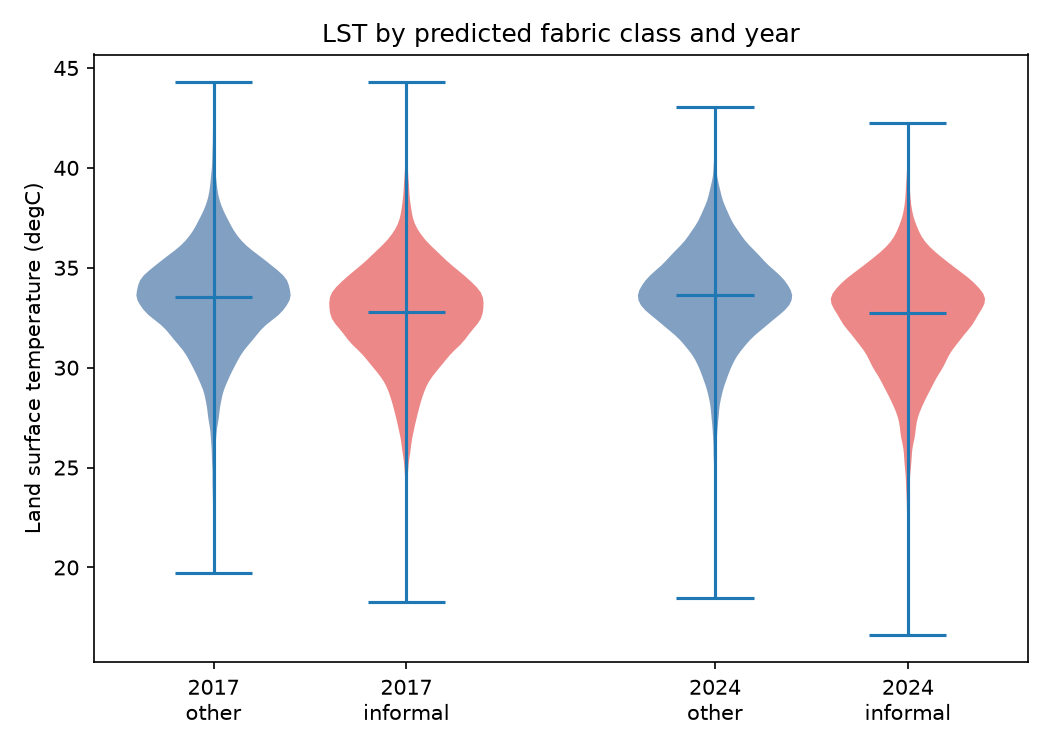
\includegraphics[width=0.62\linewidth]{figures/lst_by_class_year.png}
\caption{The daytime result. Each shape shows the spread of temperatures for a
class (red = informal, blue = other). Informal sits slightly \emph{lower} ---
the opposite of a heat penalty. Section~\ref{sec:night} shows this reverses at
night.}
\end{figure}

% ---------------- 7. Extension ----------------
\section{Extension: does the penalty appear at night?}\label{sec:night}
The daytime null has an obvious suspect --- \textbf{time of day}. Heat inequity
is largely a \emph{nighttime} problem: dense fabric soaks up sun all day and
radiates it back after dark, exactly when people without air-conditioning are
trying to sleep. But Landsat only passes over at $\sim$10:30 am. So I re-ran
the analysis on MODIS \textbf{night} temperature, with MODIS \textbf{day} as a
same-satellite control.

\paragraph{The daytime cooling reverses at night.} Landsat-day and MODIS-day
agree almost exactly (both $-0.45$\dC{} in 2017), which rules out a ``different
satellite'' excuse --- and then the \emph{same} MODIS sensor turns positive at
night:

\begin{table}[htbp]
\centering
\small
\begin{tabular}{@{}lcccc@{}}
\toprule
Year & Landsat day & MODIS day & MODIS \textbf{night} & day$\rightarrow$night shift \\
\midrule
2017 & $-0.445$\dC & $-0.446$\dC & \textbf{$+0.298$\dC} & \textbf{$+0.74$\dC} \\
2024 & $-0.380$\dC & $-0.205$\dC & \textbf{$-0.075$\dC} & $+0.31$\dC \\
\bottomrule
\end{tabular}
\caption{Adjusted informal effect by time of day and sensor. In both years the
effect moves toward hotter from day to night.}
\end{table}

In 2017 it crosses zero into a real nighttime \textbf{heat penalty}
($+0.30$\dC).

\begin{figure}[htbp]
\centering
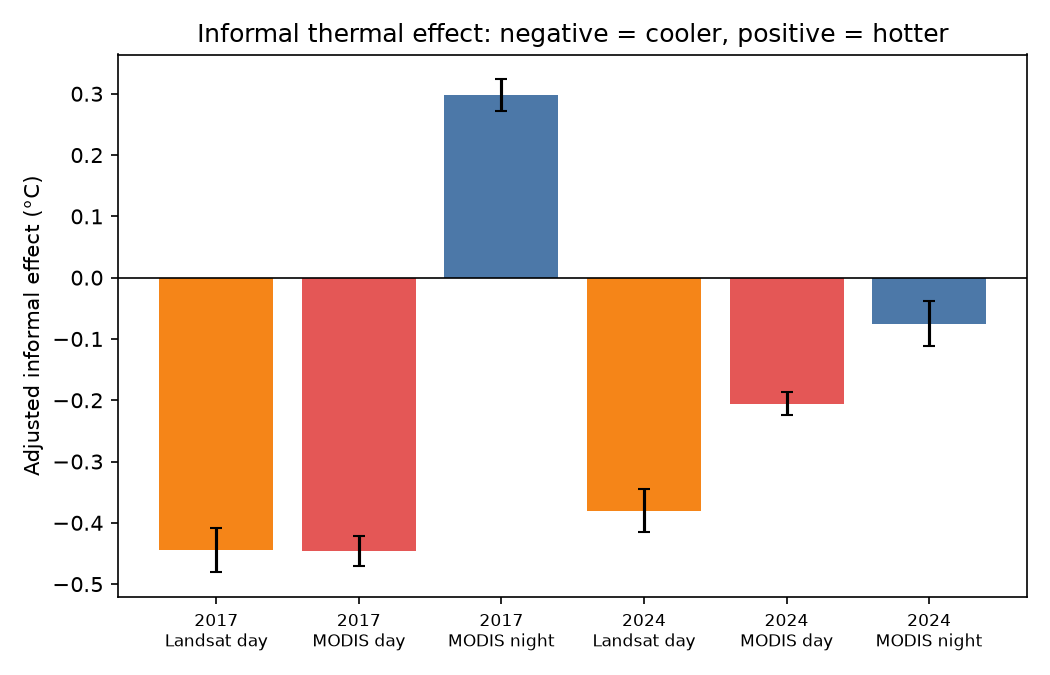
\includegraphics[width=0.7\linewidth]{figures/day_vs_night_effect.png}
\caption{The key result. Bars below zero (orange/red) mean informal is cooler;
above zero (blue) means hotter. Daytime satellites agree informal is cooler ---
but the same MODIS sensor at night flips positive in 2017, the fingerprint of
heat trapped overnight.}
\end{figure}

\paragraph{The ``pure-cell'' test sharpens 2017.} Using only 1 km cells that
are $\geq$70\% one fabric (so we compare clean examples, not mixtures),
informal cells are \textbf{$+1.13$\dC{} hotter at night} than other cells in
2017 (95\% CI $[+0.80, +1.46]$, $p \approx 2\times10^{-11}$; 97 informal vs 947
other cells). The 2024 pure-cell contrast is flat --- which the next test
explains.

\paragraph{Why 2024 washes out: core vs fringe.} Splitting the 2024
pure-informal cells by whether they were \emph{already} informal in 2017
(established \textbf{core}) or appeared only by 2024 (\textbf{expansion}), and
comparing each to other cells on night temperature:

\begin{table}[htbp]
\centering
\small
\begin{tabular}{@{}lcccc@{}}
\toprule
Group & cells & adjusted night gap vs other & 95\% CI & $p$ \\
\midrule
\textbf{Core (established)} & 164 & \textbf{$+0.34$\dC} & $[-0.01, +0.69]$ & 0.059 \\
Expansion (new fringe) & 60 & $-0.14$\dC & $[-0.67, +0.39]$ & 0.60 \\
\bottomrule
\end{tabular}
\caption{2024 nighttime gap for established core vs newly-expanded fringe.}
\end{table}

\begin{figure}[htbp]
\centering
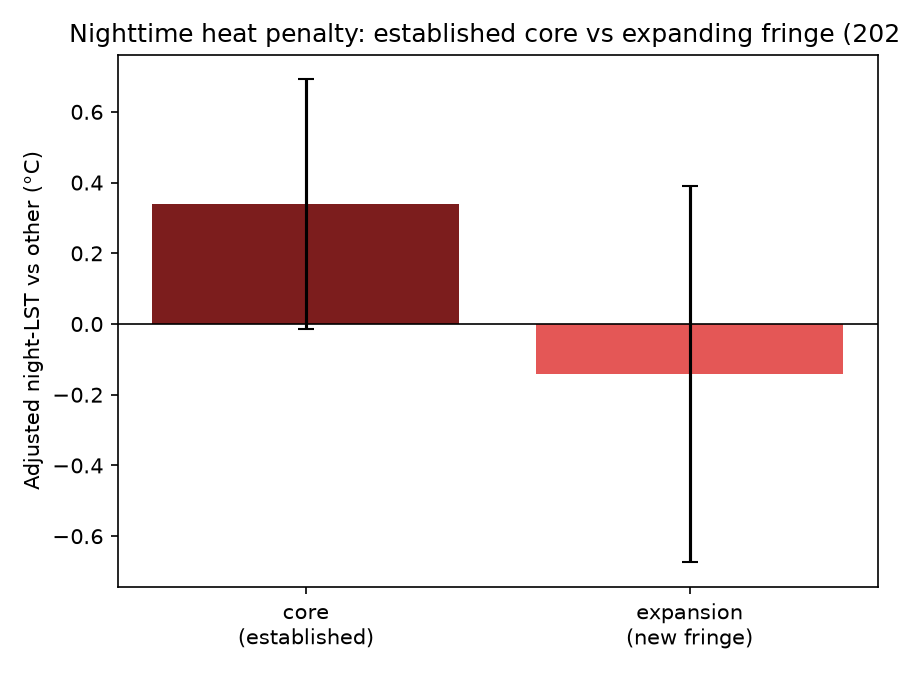
\includegraphics[width=0.6\linewidth]{figures/core_vs_fringe_night.png}
\caption{The 2024 nighttime heat gap for established core informal vs the
newly-built fringe. The core trends hotter ($+0.34$\dC, marginal at
$p=0.06$); the new fringe shows nothing --- consistent with newer,
lower-density housing not yet packed tightly enough to trap heat overnight.}
\end{figure}

The core effect is marginal ($p=0.06$, only 164 cells), so I don't overstate
it --- but its \emph{direction} is clear, and mixing in the penalty-free
expansion cells is exactly what flattens the 2024 average. Together --- a
strong, significant 2017 night penalty and a core-concentrated 2024 signal ---
the nighttime evidence supports the reading that daytime satellites simply
couldn't see the heat burden.

% ---------------- 8. Discussion ----------------
\section{Discussion}
The story is a twist with a resolution. By day, a strong classifier finds
\textbf{no heat penalty} --- informal fabric even reads slightly cooler. But
that's about the \emph{measurement}, not the settlements. At 10:30 am, dense
low-rise informal fabric with narrow shaded alleys stays cool, while the
``formal'' side is full of hot open surfaces --- big metal roofs, wide roads,
bare lots. Switch to \textbf{night}, and the sign flips: informal fabric runs
hotter, most clearly in the established dense core where decades of packed
building have built up heat-holding mass. Daytime surface temperature is the
wrong instrument for a problem that is fundamentally nocturnal --- the penalty
was there all along, hidden by the hour of the overpass. That it concentrates
in the core rather than the fringe is itself telling: the heat burden is a
property of mature, consolidated informal fabric, and the frontier may be
growing into it.

% ---------------- 9. Limitations ----------------
\section{Limitations}
\begin{itemize}[leftmargin=1.4em, itemsep=1pt]
  \item \textbf{Surface $\neq$ air temperature.} Both satellites measure
  surface heat, not the air people breathe. The night result is a better proxy
  for lived experience, but still a proxy.
  \item \textbf{MODIS is coarse.} At 1 km the night analysis mixes fabric
  types; the pure-cell and core/fringe tests reduce but can't remove this, and
  the 2024 core effect is marginal ($p=0.06$).
  \item \textbf{Resolution ceiling.} 30 m (day) / 1 km (night) temperature vs
  10 m fabric --- no claim about individual buildings.
  \item \textbf{Hand-drawn labels.} 70 polygons, my own judgement, no field
  survey; pushing toward 100--150 would tighten the estimates.
  \item \textbf{Association, not proof.} These are correlations after controls,
  not a demonstrated mechanism.
  \item \textbf{One city, one season.} Dry-season Addis only; results won't
  automatically transfer elsewhere.
\end{itemize}

% ---------------- 10. Conclusion ----------------
\section{Conclusion}
An AI satellite model maps Addis Ababa's informal fabric well (94\% AUC) and
cleanly tracks its growth --- a real advance over hand-crafted indices, and one
that reaches the fringe official-boundary studies miss. The thermal lesson is
the payoff: by day, informal fabric shows \emph{no} heat penalty and even looks
cooler, but that is an artifact of the mid-morning overpass. At \textbf{night}
the penalty appears --- informal fabric runs up to $\sim$1\dC{} hotter,
concentrated in the established dense core --- exactly where heat harms people
who can't cool down after dark. The takeaway generalizes well beyond Addis:
\textbf{whether you detect urban-heat inequity depends on the time of day you
measure it}, and daytime surface temperature can hide a penalty that is plainly
there at night. Measuring at night --- and eventually air temperature --- is
the necessary next step.

\end{document}
